
\documentclass{article}

\usepackage{fancyhdr} % Required for custom headers
\usepackage{lastpage} % Required to determine the last page for the footer
\usepackage{extramarks} % Required for headers and footers
\usepackage[usenames,dvipsnames]{color} % Required for custom colors
\usepackage{graphicx} % Required to insert images
\usepackage{listings} % Required for insertion of code
\usepackage{courier} % Required for the courier font
\usepackage{lipsum} % Used for inserting dummy 'Lorem ipsum' text into the template
\usepackage{caption}
\usepackage{subcaption}
\usepackage{amsmath}
\usepackage[utf8]{inputenc}

\graphicspath{ {figures} }

% Margins
\topmargin=-0.45in
\evensidemargin=0in
\oddsidemargin=0in
\textwidth=6.5in
\textheight=9.0in
\headsep=0.25in

\linespread{1.1} % Line spacing

% Set up the header and footer
\pagestyle{fancy}
\lhead{\hmwkAuthorName} % Top left header
\chead{\hmwkClass\ (\hmwkClassInstructor\ \hmwkClassTime): \hmwkTitle} % Top center head
\rhead{\firstxmark} % Top right header
\lfoot{\lastxmark} % Bottom left footer
\cfoot{} % Bottom center footer
\rfoot{Page\ \thepage\ of\ \protect\pageref{LastPage}} % Bottom right footer
\renewcommand\headrulewidth{0.4pt} % Size of the header rule
\renewcommand\footrulewidth{0.4pt} % Size of the footer rule

\setlength\parindent{0pt} % Removes all indentation from paragraphs

%----------------------------------------------------------------------------------------
%	CODE INCLUSION CONFIGURATION
%----------------------------------------------------------------------------------------

\definecolor{MyDarkGreen}{rgb}{0.0,0.4,0.0} 
\lstloadlanguages{Matlab}
\lstset{language=Matlab,
        frame=single,
        basicstyle=\small\ttfamily,
        keywordstyle=[1]\color{Blue}\bf,
        keywordstyle=[2]\color{Purple},
        keywordstyle=[3]\color{Blue}\underbar,
        identifierstyle=,
        commentstyle=\usefont{T1}{pcr}{m}{sl}\color{MyDarkGreen}\small, 
        stringstyle=\color{Purple},
        showstringspaces=false,
        tabsize=5, 
        morekeywords={rand},
        morekeywords=[2]{on, off, interp},
        morekeywords=[3]{test},
        morecomment=[l][\color{Blue}]{...},
        numbers=left,
        firstnumber=1,
        numberstyle=\tiny\color{Blue},
        stepnumber=5
}

% Creates a new command to include a perl script, the first parameter is the filename of the script (without .pl), the second parameter is the caption
\newcommand{\matlabscript}[2]{
\begin{itemize}
\item[]\lstinputlisting[caption=#2,label=#1]{#1.m}
\end{itemize}
}

%----------------------------------------------------------------------------------------
%	DOCUMENT STRUCTURE COMMANDS
%	Skip this unless you know what you're doing
%----------------------------------------------------------------------------------------

% Header and footer for when a page split occurs within a problem environment
\newcommand{\enterProblemHeader}[1]{
\nobreak\extramarks{#1}{#1 continued on next page\ldots}\nobreak
\nobreak\extramarks{#1 (continued)}{#1 continued on next page\ldots}\nobreak
}

% Header and footer for when a page split occurs between problem environments
\newcommand{\exitProblemHeader}[1]{
\nobreak\extramarks{#1 (continued)}{#1 continued on next page\ldots}\nobreak
\nobreak\extramarks{#1}{}\nobreak
}

\setcounter{secnumdepth}{0} % Removes default section numbers
\newcounter{homeworkProblemCounter} % Creates a counter to keep track of the number of problems

\newcommand{\homeworkProblemName}{}
\newenvironment{homeworkProblem}[1][Problem \arabic{homeworkProblemCounter}]{ % Makes a new environment called homeworkProblem which takes 1 argument (custom name) but the default is "Problem #"
\stepcounter{homeworkProblemCounter} % Increase counter for number of problems
\renewcommand{\homeworkProblemName}{#1} % Assign \homeworkProblemName the name of the problem
\section{\homeworkProblemName} % Make a section in the document with the custom problem count
\enterProblemHeader{\homeworkProblemName} % Header and footer within the environment
}{
\exitProblemHeader{\homeworkProblemName} % Header and footer after the environment
}

\newcommand{\problemAnswer}[1]{ % Defines the problem answer command with the content as the only argument
\noindent\framebox[\columnwidth][c]{\begin{minipage}{0.98\columnwidth}#1\end{minipage}} % Makes the box around the problem answer and puts the content inside
}

\newcommand{\homeworkSectionName}{}
\newenvironment{homeworkSection}[1]{ % New environment for sections within homework problems, takes 1 argument - the name of the section
\renewcommand{\homeworkSectionName}{#1} % Assign \homeworkSectionName to the name of the section from the environment argument
\subsection{\homeworkSectionName} % Make a subsection with the custom name of the subsection
\enterProblemHeader{\homeworkProblemName\ [\homeworkSectionName]} % Header and footer within the environment
}{
\enterProblemHeader{\homeworkProblemName} % Header and footer after the environment
}

%----------------------------------------------------------------------------------------
%	NAME AND CLASS SECTION
%----------------------------------------------------------------------------------------

\newcommand{\hmwkTitle}{Assignment\ \#4}
\newcommand{\hmwkDueDate}{Monday,\ September\ 11,\ 2017}
\newcommand{\hmwkClass}{Pattern Recognition} % Course/class
\newcommand{\hmwkClassTime}{09:10am} % Class/lecture time
\newcommand{\hmwkClassInstructor}{shkim} % Teacher/lecturer
\newcommand{\hmwkAuthorName}{Tien Anh Nguyen} % Your name

%----------------------------------------------------------------------------------------
%	TITLE PAGE
%----------------------------------------------------------------------------------------

\title{
\vspace{2in}
\textmd{\textbf{\hmwkClass:\ \hmwkTitle}}\\
\normalsize\vspace{0.1in}\small{Due\ on\ \hmwkDueDate}\\
\vspace{0.1in}\large{\textit{\hmwkClassInstructor\ \hmwkClassTime}}
\vspace{3in}
}

\author{\textbf{\hmwkAuthorName}}
\date{} % Insert date here if you want it to appear below your name

%----------------------------------------------------------------------------------------

\begin{document}

\maketitle

%----------------------------------------------------------------------------------------
%	TABLE OF CONTENTS
%----------------------------------------------------------------------------------------

%\setcounter{tocdepth}{1} % Uncomment this line if you don't want subsections listed in the ToC

\newpage
\tableofcontents
\newpage

%----------------------------------------------------------------------------------------
%	PROBLEM 1
%----------------------------------------------------------------------------------------

% To have just one problem per page, simply put a \clearpage after each problem

\begin{homeworkProblem}
\maketitle
\subsection{Exercise 6.3.1}
\matlabscript{mfiles/exercise_06_03_01}{Source codes}

\newpage

In the codes, we do the following tasks:
\begin{itemize}
 \item Loading training data which is stored in \textbf{DOHMMTrainingData.mat}. It is a cell array, \
      with each cell containing a string of Hs and Ts, and is interpreted as a symbol sequence of the \
      training set. For example: \textbf{HHHHTTHHTTTHTTHHHHTTHTHHHTHHHHTHHTTTHTHTHHH}.

 \item Converting each string will be converted to a sequence of symbol IDs and stored in a new cell \
      array, NumericData. \textbf{1} stands for heads and \textbf{2} for tails.

 \item Initialize the HMM with the set of values.
      \begin{equation}
          \pi = [0.6 0.4]^T;\ 
            A = \begin{bmatrix}0.6 & 0.4 \\ 0.01 & 0.99\end{bmatrix};\ 
            B = \begin{bmatrix}0.6 & 0.01 \\ 0.4 & 0.99\end{bmatrix};\ 
      \end{equation}

 \item Using function MultSeqTrainDoHMMBWsc to train the HMM with the Baum-Welch training algorithm.
 \item Function MultSeqTrainDoHMMBWsc implements the scaled version of the Baum-Welch training algorithm,\
      which stops iterating when the sum of recognition probabilities of the training sequences ceases to\
      increase.
 \item \textbf{maxEpoch} defines the maximum number of iterations during the training stage.
 \item \textbf{SumRecProbs\_1} is a vector whose ith element is the sum of recognition probabilities \
      at the ith iteration of the training algorithm.
\end{itemize}

We got the result:
\begin{itemize}
 \item number of iterations: \textbf{1000}.
 \item $\pi = [1.0000\ 0.0000]^T$
 \item $ A = \begin{bmatrix}0.9352 & 0.0648 \\ 0.9660 & 0.0340\end{bmatrix}$
 \item $ B = \begin{bmatrix} 0.6682 & 0.1006 \\ 0.3318 & 0.8994\end{bmatrix}$
\end{itemize}

Since the $\pi(1)\ =\ 1$, the first state will always be the starting one. The $A(2, 2) = 0.0340$ \
is very small if it compared to the $A(2, 1) = 0.9660$. In general, the initialization state is very
small imply that the respective events maybe not occur.
\end{homeworkProblem}
%----------------PROBLEM 1---------------------------------------------------------------


\newpage

%----------------------------------------------------------------------------------------
%	PROBLEM 2
%----------------------------------------------------------------------------------------
\begin{homeworkProblem}
\maketitle
\subsection{Exercise 6.3.2}
\matlabscript{mfiles/exercise_06_03_02}{Source codes}
\begin{itemize}
 \item Viterbi score 1 = -2.088426495300448e+03
 \item Viterbi score 2 = -1.387604868684983e+03
\end{itemize}
\end{homeworkProblem}
%----------------PROBLEM 2---------------------------------------------------------------

%----------------------------------------------------------------------------------------
%	PROBLEM 3
%----------------------------------------------------------------------------------------
\begin{homeworkProblem}
\maketitle
\subsection{Exercise 5.2.1}
\matlabscript{mfiles/exercise_05_02_01}{Source codes}

\newpage

\begin{figure}[h]
\centering
    \begin{subfigure}[h]{0.5\textwidth}
        \centering
        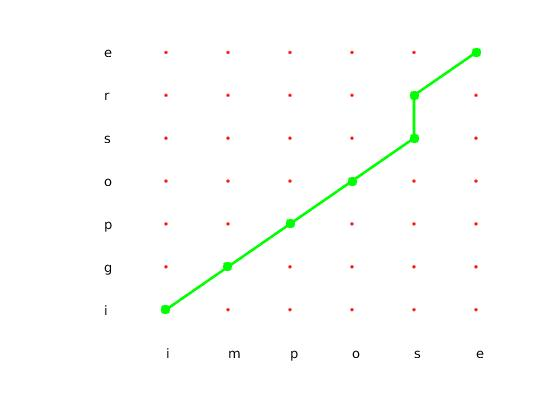
\includegraphics[width=4in,height=3in]{figures/figure_05_02_01_01.jpg}
        \caption{Optimal matching path between "impose" and "igposre"}
    \end{subfigure}\\
    \begin{subfigure}[h]{0.5\textwidth}
        \centering
        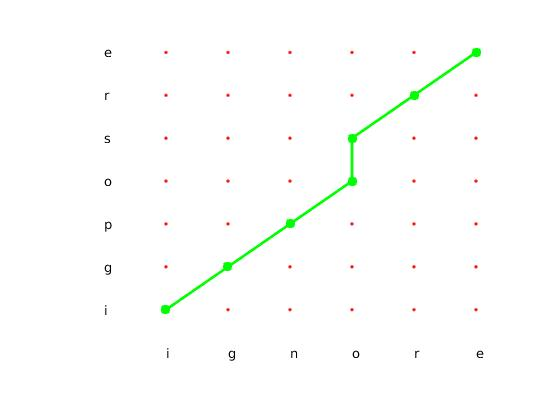
\includegraphics[width=4in,height=3in]{figures/figure_05_02_01_02.jpg}
        \caption{Optimal matching path between "ignore" and "igposre"}
    \end{subfigure}\\
\end{figure}

\begin{figure}[h]
\centering
    \begin{subfigure}[h]{0.5\textwidth}
        \centering
        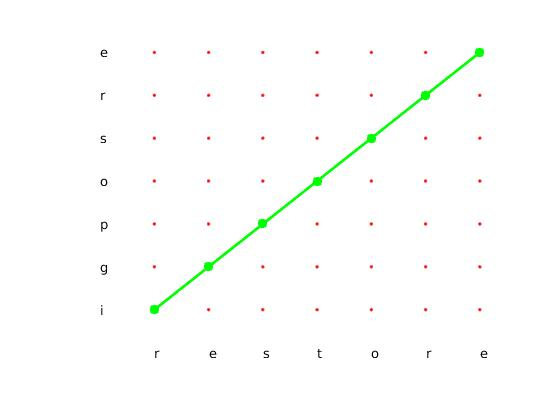
\includegraphics[width=4in,height=3in]{figures/figure_05_02_01_03.jpg}
        \caption{Optimal matching path between "restore" and "igposre"}
    \end{subfigure}\\
\end{figure}

\end{homeworkProblem}
%----------------PROBLEM 3---------------------------------------------------------------

\end{document}
